\documentclass[conference]{IEEEtran}

% Packages
\usepackage[utf8]{inputenc}
\usepackage[english]{babel}
\usepackage{amsmath}
\usepackage{amsfonts}
\usepackage{amssymb}
\usepackage{amsthm}
\usepackage{pdfpages}
\usepackage{graphicx}
\usepackage{epstopdf}
\usepackage{listings}
\usepackage{cite}
\usepackage{enumerate}
\usepackage{scientific}
\usepackage[colorlinks=false]{hyperref}
\usepackage{bookmark}

\usepackage[]{mcode}	%Matlab Code
\usepackage{tikz,pgfplots}	%Tikz

\usepgfplotslibrary{external} 
\tikzexternalize
\tikzsetexternalprefix{ext/}

% Bookmark Setup
\bookmarksetup{numbered}

% PDF Setup
\hypersetup{pdftitle={Homework 5}, pdfsubject={Documentation of 5th Homework}, pdfauthor={Stefan Röhrl}, pdfkeywords={Neuroprothetik Exercise}, pdfcreator={LaTeX}, hidelinks}


\begin{document}
%
% cite all references
%\nocite{*}
%
% paper title
% can use linebreaks \\ within to get better formatting as desired
\title{Homework 5\\ Multicompartment Model}

\author{\IEEEauthorblockN{Stefan Röhrl}
\IEEEauthorblockA{Technische Universität München, Arcisstraße 21, Munich, Germany\\
Email: stefan.roehrl@tum.de}}

% use for special paper notices
%\IEEEspecialpapernotice{(Invited Paper)}

% make the title area
\maketitle

\IEEEpeerreviewmaketitle

\section{Create a Multicompartment Model}
Das Multicompartment Modell wurde durch Einfügen einer zusätzlichen Dimension in alle Variablen umgesetzt. Die neuen Spannungswerte werden wie in den Hausaufgaben Folien vorgeschlagen durch lösen eines Gleichungssystems berechnet.

\begin{lstlisting}
    % Berechnen Membranspannung
    B = V(:,k)+dt/c * (-sum(i_ion(:,k,:),3)...
        + iStimulus(:,k));
    A = (eye(comparts) - dt/(c * Ra) * C);
    V(:,k+1) = A\B;
\end{lstlisting}

\section{Experiments}

\begin{enumerate}

\item Die Anregung mit einem 5ms langen Puls mit einer Amplitude von $10\frac{\mu A}{cm^2}$ führt zu folgendem Verlauf der Membranpotentiale jedes Compartments. 

\begin{figure}[h]
	\centering
	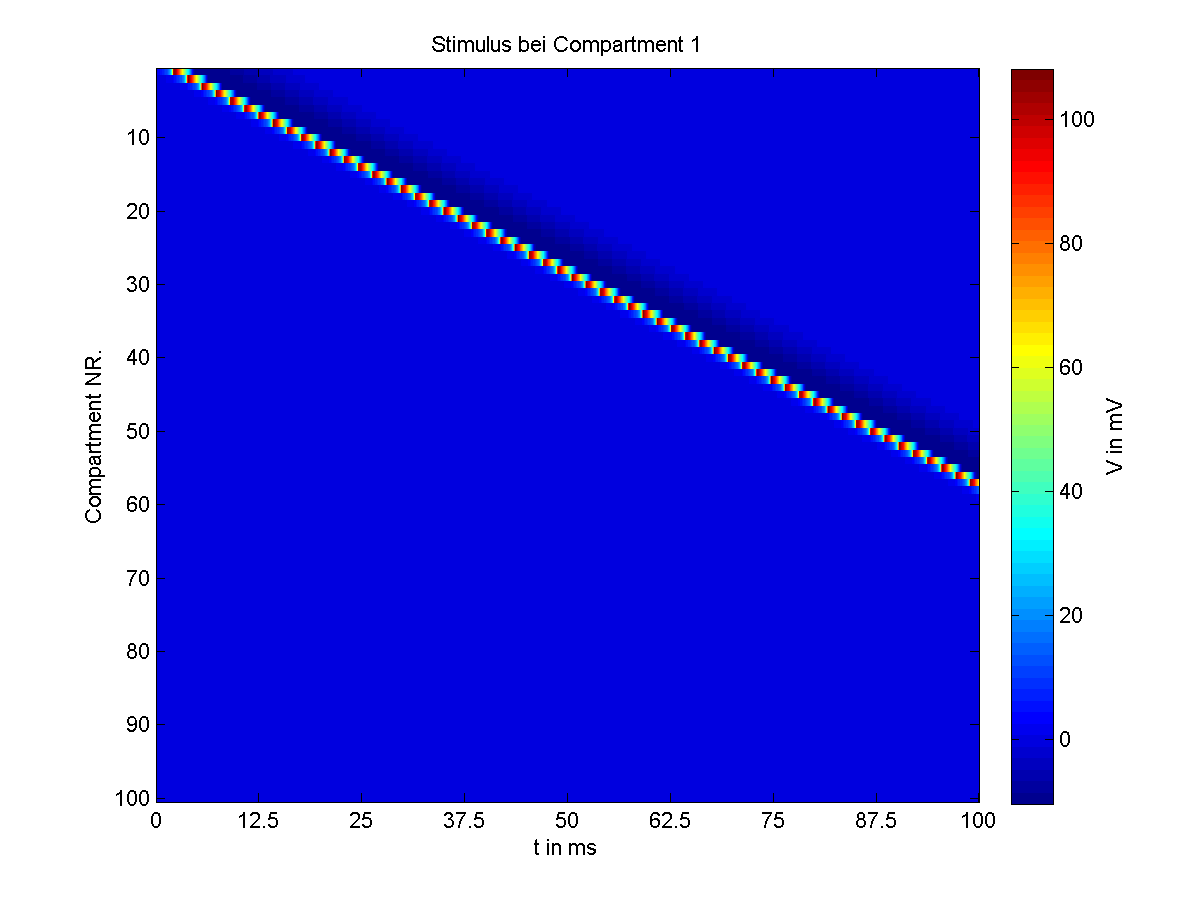
\includegraphics[width=0.5\textwidth]{img/compart1.png}
	\caption{Anregung an Compartment 1}
	\label{fig:compart1}
\end{figure}

\end{enumerate}

\end{document}


